\documentclass{article}
\usepackage{graphicx} % Required for inserting images

\title{Assignment 2 - HyperLogLog}
\author{
        Andreas Vinkler \\ \textit{anmv@itu.dk} \\ \\
    Frederik Orth Kølbel \\ \textit{frek@itu.dk} \\ \\
    Tobias Lysdal Hansen \\ \textit{tolh@itu.dk} \\ \\
    }
\date{October 2024}

\begin{document}

\maketitle
\newpage


\section{Introduction}
This report explores, implements and tests a variation of a \textit{HashSet} method and the \textit{HyperLogLog} algorithm. We intend to investigate differences between these two ways of solving for distinct elements.
(add more later)

\section{Implementation}
Our implementation started with testing out our \textit{HashSet}, or rather our hash function for a \textit{Hash} Method on n distinct elements. Theoretically, the \textit{HashSet} mehtod is a good solution when dealing with tracking and storing distinct elements, as the initialization is linear based \textit{n}, so $\mathcal{O}(m)$ which then allows for constant time $\mathcal{O}(1)$ access to the elements. However, while this does satisfy as a "good" solution time complexity wise, the \textit{HashSet} method ends up running into space complexity issues, as \textit{n} becomes sufficiently large. \textbf{bad sentence reiterate}This is due to the \textit{Hash} method keeps trying to optimize and allocate memory to the elements, even though it cannot fully make room for it. Consequently, a \textit{Hash} method does not fulfill our time and space complexity restraints.
We initiated our variants by implementing the hash function. 
\\

\textbf{Cut and/or add stuff. In-depth about storing data in an Array m (register)}
We then extended our functioning hashing method for our \textit{HyperLogLog} implementation. The \textit{HyperLogLog} algorithm works, in short, with a hashing function and in conjunction with a function \textit{p} to estimate the cardinality of an array based on the number of leading zeros when the input is in a binary representation. Given that the cardinality is estimated based on a set of uniformly distributed random numbers, variance can occur. We reduce the overall variance of the estimation by tracking the maximum number of leading zeros in numerous subsets of our original set of distinct elements, which is then supported by utilizing the harmonic mean. Consequently, we can find the an overall estimation for the whole set.
The \textit{HyperLogLog} should theoretically work in $\mathcal{O}(m)$ time complexity and with $\mathcal{O}(m)$ space complexity.
\\

add few lines about our tests. The 1-1million elements
\\

2.75% "expected standard error"
1027528 for 1mil distinct elements
excepted error range for m = 1024

\section{Experiments / Findings}
All tests were done on x and y(include Frederiks' and Andreas' laptop specs.)
Firstly, we tested the accuracy or our function \textit{p}. As can be observed via our Figure \ref{fig:functionP} showcasing the distribution of leading zeros on an input size of 1million \textit{n}  on the y-axis and number of leading zeros on the x-axis. As we continue iterating, the probability of the estimation being a non-zero decreases. However, outliers can affect the results. This can be one explanation as to why our function \textit{p} accurately estimates the distribution, but becomes less accurate as \textit{number of leading zeros} increase.

Consider mentioning our hash function evaluation

Additionally, we 





\begin{figure} [hbt!]
    \centering
    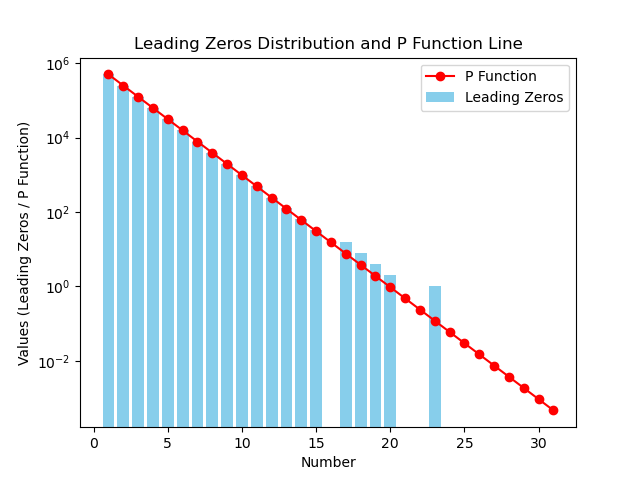
\includegraphics[width=\textwidth]{QualityTestHistogram.png}
    \caption{Historgram depicting the accuracy of our function \textit{p}}
    \label{fig:functionP} 
\end{figure}



\end{document}
